% ---------------------------------------------------------------------------
% Hybrid Sparse-Dense Retrieval with Cross-Encoder Reranking
% Compile:  pdflatex main && bibtex main && pdflatex main && pdflatex main
% Uses only standard packages, so it builds on a plain TeX Live / MiKTeX install.
% ---------------------------------------------------------------------------
\documentclass[10pt,twocolumn]{article}

\usepackage[margin=0.75in]{geometry}
\usepackage[T1]{fontenc}
\usepackage[utf8]{inputenc}
\usepackage{times}
\usepackage{graphicx}
\usepackage{booktabs}
\usepackage{amsmath}
\usepackage{url}
\usepackage[hidelinks]{hyperref}
\usepackage{caption}
\captionsetup{font=small,labelfont=bf}

\title{\bf Hybrid Sparse--Dense Retrieval with Cross-Encoder Reranking\\
for Domain-Specific Question Answering}

\author{
  Vivansh Garg\\
  \small B.Tech Computer Science and Engineering (Data Science), Third Year\\
  \small \texttt{vivanshgarg05@gmail.com}
  % TODO: add institution name, course code (Deep Learning), and supervisor
}
\date{\today}

\begin{document}
\maketitle

% ===========================================================================
\begin{abstract}
% 150--200 words. Write this LAST, after the numbers are in.
% Formula: problem -> why existing methods fall short -> what you built ->
%          what you measured -> the single most surprising number -> what it means.
Retrieval-augmented question answering over a specialised corpus depends on
finding the right evidence, and no single retrieval method finds it reliably:
lexical matching handles exact terminology but breaks under paraphrase, while
dense retrieval handles paraphrase but loses rare identifiers. We present a
multi-stage pipeline that runs BM25 and a dense bi-encoder independently, merges
their ranked lists with Reciprocal Rank Fusion, and rescores the fused pool with
a Transformer cross-encoder before answering. Evaluating on SciFact
(\textsc{beir}), we isolate the contribution of each stage through a four-way
ablation and report accuracy against latency and index cost.
% TODO: fill in from results/metrics.json
Fusion improves nDCG@10 over the stronger single retriever by \textbf{XX} points,
and reranking a pool of $N{=}50$ candidates adds a further \textbf{YY} points at a
cost of \textbf{ZZ}\,ms per query. A manual analysis of \textbf{NN} residual
failures attributes them chiefly to terminology mismatch and to evidence that is
absent from the corpus rather than mis-ranked.
\end{abstract}

% ===========================================================================
\section{Introduction}
\label{sec:intro}

% 3--4 paragraphs.
% P1  The setting: QA over a specialised corpus, answers must be grounded and cited.
% P2  The tension: BM25 vs dense, with a concrete example of each failing.
%     (Pull a real one from results/failure_analysis.csv once you have it.)
% P3  What this paper does: the pipeline, in one sentence per stage.
% P4  Contributions, as an explicit list.

\noindent Our contributions are:
\begin{enumerate}\itemsep2pt
  \item A reproducible multi-stage retrieval pipeline (BM25 $+$ dense $\rightarrow$
        RRF $\rightarrow$ cross-encoder $\rightarrow$ grounded answer) with a single
        configuration file controlling every stage.
  \item A controlled four-way ablation --- sparse, dense, fusion, fusion$+$reranking ---
        over one fixed corpus, index and query set, isolating what each stage contributes.
  \item A cost-aware evaluation that reports accuracy jointly with query latency,
        index size and reranking depth, rather than accuracy alone.
  \item A manual failure analysis over the residual errors, categorised into
        terminology mismatch, query ambiguity, missing and conflicting evidence.
\end{enumerate}

% ===========================================================================
\section{Related Work}
\label{sec:related}

% Four short paragraphs, one per thread. Two to four citations each; do not pad.
\paragraph{Sparse retrieval.} BM25~\cite{robertson2009bm25} remains a strong
baseline on out-of-domain collections; learned sparse models such as
SPLADE~\cite{formal2021splade} keep the inverted index while learning term weights.

\paragraph{Dense retrieval.} DPR~\cite{karpukhin2020dpr} and
Contriever~\cite{izacard2022contriever} embed queries and passages into a shared
space. BEIR~\cite{thakur2021beir} showed that these models often lose to BM25 under
domain shift --- the observation this work builds on.

\paragraph{Fusion and reranking.} Reciprocal Rank Fusion~\cite{cormack2009rrf}
combines ranked lists without score calibration. Cross-encoders trained on
MS MARCO~\cite{nogueira2019passage} rescore a shallow candidate pool; monoT5 and
related work~\cite{nogueira2020document} push this further.

\paragraph{Retrieval-augmented generation.} RAG~\cite{lewis2020rag} and
FiD~\cite{izacard2021fid} condition generation on retrieved passages; attribution
and citation faithfulness remain open~\cite{gao2023enabling}.

% ===========================================================================
\section{Method}
\label{sec:method}

\subsection{Corpus preparation}
% Chunking strategy and why. Report the resulting chunk count and chunks/doc from
% results/metrics.json ("corpus" block).

\subsection{Stage 1: sparse retrieval}
BM25 scores a query--passage pair as
\begin{equation}
\mathrm{BM25}(q,d)=\sum_{t \in q}\mathrm{IDF}(t)\,
\frac{f(t,d)\,(k_1+1)}{f(t,d)+k_1\!\left(1-b+b\frac{|d|}{\mathrm{avgdl}}\right)},
\end{equation}
with $k_1={\tt TODO}$ and $b={\tt TODO}$. % state your config values
% One sentence on what this stage is good at: exact terms, codes, rare entities.

\subsection{Stage 2: dense retrieval}
% Bi-encoder name, dimensionality, pooling, normalisation, index type.
% Make the independence explicit: E(q) and E(d) never see each other.

\subsection{Stage 3: rank fusion}
Reciprocal Rank Fusion~\cite{cormack2009rrf} scores a document by
\begin{equation}
\mathrm{RRF}(d)=\sum_{s \in S} \frac{w_s}{k + \mathrm{rank}_s(d)},
\end{equation}
where $\mathrm{rank}_s(d)$ is $d$'s position in system $s$'s list and $k$
damps the influence of the very top ranks. Fusing \emph{ranks} rather than scores
sidesteps the incompatibility between unbounded BM25 scores and bounded cosine
similarities.
% State k and weights. Reference the sweep in results/sweep_rrf_k.json to show the
% result is not an artefact of one k.

\subsection{Stage 4: cross-encoder reranking}
% [CLS] q [SEP] p [SEP], full cross-attention, one forward pass per pair.
% State the model, the candidate depth N, and that cost is O(N) per query.

\subsection{Stage 5: grounded answering}
% Prompt, number of passages, citation format, abstention behaviour.

% ===========================================================================
\section{Experimental Setup}
\label{sec:setup}

\paragraph{Dataset.} SciFact~\cite{wadden2020scifact} as distributed in
BEIR~\cite{thakur2021beir}: 5{,}183 scientific abstracts and 300 test claims with
document-level relevance judgements.
% State judged queries actually evaluated and mean gold docs per query.

\paragraph{Models.} % bi-encoder, cross-encoder, reader, with exact HF identifiers.

\paragraph{Hardware.} % GPU model, VRAM, CUDA version. Latency numbers are meaningless without it.

\paragraph{Metrics.} Recall@$k$ and Precision@$k$ measure whether the evidence
was found; MRR measures how early; nDCG@$k$ is graded and rank-discounted and is
our primary metric. Relevance is judged at document level, so chunk rankings are
collapsed to their parent documents before scoring. Answers are scored on
correctness, completeness, faithfulness and citation accuracy.
% State the manual annotation protocol: how many answers, who annotated, what scale.

\paragraph{Significance.} Differences are tested with a two-sided paired
bootstrap over per-query nDCG@10 ($10^4$ resamples).

% ===========================================================================
\section{Results}
\label{sec:results}

\begin{table}[t]
\centering\small
\caption{Retrieval ablation on SciFact. All variants share one corpus, one
chunking and one index; only the retrieval strategy differs.}
\label{tab:ablation}
\begin{tabular}{lccccr}
\toprule
Variant & nDCG@10 & R@10 & R@100 & MRR@10 & ms/q \\
\midrule
BM25            & & & & & \\
Dense           & & & & & \\
RRF fusion      & & & & & \\
\; $+$ reranking & & & & & \\
\bottomrule
\end{tabular}
% Fill from results/ablation.csv. Bold the best cell per column.
\end{table}

\begin{figure}[t]
\centering
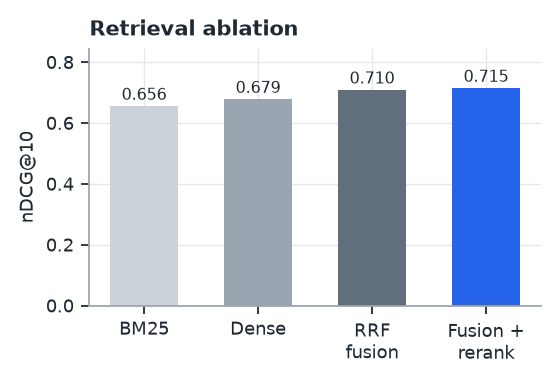
\includegraphics[width=\columnwidth]{figures/ablation_ndcg.png}
\caption{nDCG@10 by variant.}
\label{fig:ablation}
\end{figure}

\begin{figure}[t]
\centering
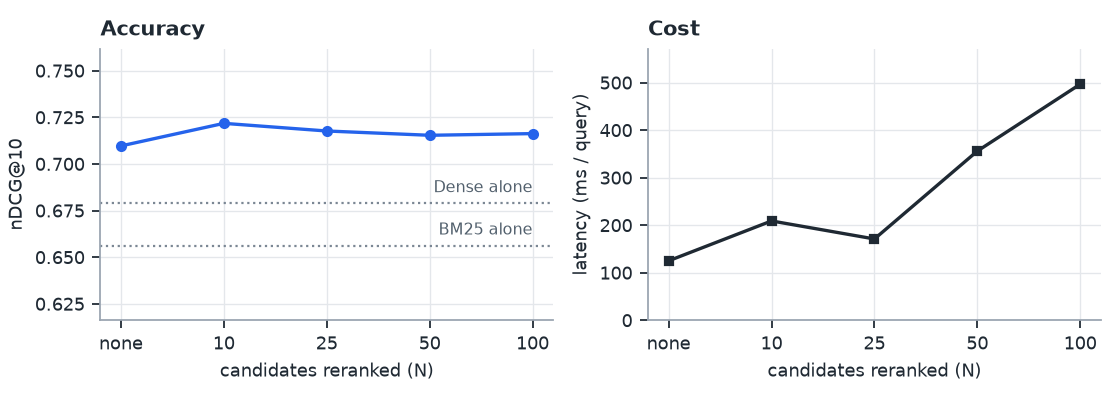
\includegraphics[width=\columnwidth]{figures/latency_accuracy.png}
\caption{Reranking depth $N$ trades latency for accuracy. % state where it saturates
}
\label{fig:latency}
\end{figure}

\subsection{Which stage helps which question?}
% The interesting part. Split queries by a property you can compute:
%   - queries containing a rare term / numeral / entity  -> expect BM25 to win
%   - queries with low lexical overlap with their gold doc -> expect dense to win
% Report the two subsets separately. This is the claim the ablation exists to support.

\subsection{Answer quality}
% Table: correctness, completeness, faithfulness, citation precision/recall.
% State n annotated and inter-annotator agreement if you had a second annotator.

\subsection{Cost}
% Index build time, index size on disk, per-query latency by stage.

% ===========================================================================
\section{Failure Analysis}
\label{sec:failures}

% Distribution over the six categories, then 2--3 verbatim examples with the query,
% the gold passage and what was retrieved instead. Concrete examples are what an
% examiner remembers.

% ===========================================================================
\section{Limitations}
\label{sec:limitations}

% Be honest and specific; this section earns marks rather than losing them.
%  - One dataset, one domain: generality is not established.
%  - Document-level judgements mean chunk-level precision is not directly measured.
%  - Off-the-shelf models; no in-domain fine-tuning of either encoder.
%  - Manual answer annotation by a single annotator, N answers.
%  - Latency measured on one machine, batch size 1, warm cache.

% ===========================================================================
\section{Conclusion}
\label{sec:conclusion}

% Three or four sentences. What you built, the one number that matters,
% and the next thing you would try.

% ===========================================================================
\section*{Reproducibility}
Code, configuration and results:
\url{https://github.com/TODO-USERNAME/hybrid-retrieval-qa}.
All experiments run from a single configuration file; every number in this paper
is regenerated by \texttt{python scripts/run\_ablation.py}.

\bibliographystyle{plain}
\bibliography{references}

\end{document}
